\documentclass[11pt, twocolumn]{report}
\usepackage[a4paper, hmargin={2.8cm, 2.8cm}, vmargin={2.5cm, 2.5cm}]{geometry}
%\usepackage[T1]{fontenc}
\usepackage[utf8]{inputenc}
\usepackage{eso-pic} % \AddToShipoutPicture
\usepackage{graphicx} % \includegraphics
\usepackage[english]{babel}
\usepackage{tcolorbox}
\usepackage{multicol}
\usepackage{amssymb}
\usepackage{amsmath}
\usepackage{fancyhdr}
\usepackage{fancyvrb}
\usepackage{geometry}
\usepackage{listings}
\usepackage[hyphens]{url}
\usepackage{breakurl}
\usepackage{cite}
\usepackage{color}
\usepackage{array}
\usepackage{multicol}
\usepackage[toc,page]{appendix}
\usepackage[breaklinks=true]{hyperref}
\usepackage{float}
\usepackage{xcolor}
\usepackage{tablefootnote}
\usepackage{footnote}
\usepackage{lipsum}
\usepackage{tocloft}

\usepackage{coffee4} % Comment me out 

%%% Macros
% easier figure
% usage: \pic{width}{image}{caption}{label} 
\newcommand\pic[4]{% these comment signs will prevent the introduction of spurious spaces
  \begin{figure}[h!]
  \centering
  \includegraphics[width=#1\textwidth]{#2}
  \caption{#3}
  \label{#4}
  \end{figure}
}




\newcolumntype{C}[1]{>{\centering\let\newline\\\arraybackslash\hspace{0pt}}m{#1}}
\setlength{\columnsep}{1cm}


\author{
  Meznik, Jan\\
  \texttt{pzj895@alumni.ku.dk}\\
  \texttt{jan@meznik.dk}
  \and
  Jacobi, Mark Jan\\
  \texttt{dcz738@alumni.ku.dk}
}

\title{
	\vspace{3cm}
	\huge{TCP/IP in hardware using SME}\\
		\vspace{0.5cm}
	\Large{Write something clever here}
}



% Header
\pagestyle{fancy}


\iffalse
\fancyhf{}
%\fancyhead[L]{}
%\fancyhead[R]{}
%\fancyhead[C]{}
%\fancyfoot[C]{Center \leftmark}
\fi

\lhead{University of Copenhagen}
%\chead{}
\rhead{TCP/IP in SME}


\begin{document}
\onecolumn


%%%%% KU HEADER %%%%%%%%%%%%%%%%%%%%%%%
\AddToShipoutPicture*{\put(0,0){\includegraphics*[viewport=0 0 700 600]{include/natbio-farve}}}
\AddToShipoutPicture*{\put(0,602){\includegraphics*[viewport=0 600 700 1600]{include/natbio-farve}}}
\AddToShipoutPicture*{\put(0,0){\includegraphics*{include/nat-en}}}
\clearpage
\maketitle
\pagenumbering{roman}
\thispagestyle{empty}
\newpage
%%%%%%%%%%%%%%%%%%%%%%%%%%%%%%%%%%%%%%%


%\begin{abstract}
\thispagestyle{empty}
%In this thesis, we design and implement a networking protocol stack in hardware
using the Synchronous Message Exchange model -- a new framework intended to
help model hardware descriptions.  The final pipelined design boasts with
a decentralized memory model, with model division easily extensible and
modifiable, closely ressembling that of the architecture of the Internet
Protocol Suite.

Initial tests performed on the simulated system with real captured network
traffic suggests stability, promising protocol compliance, and an acceptable, but
theoretical, performance. Numerous suggestions are discussed to improve the performance,
such as widening the bus-widths or replicating the stack itself to multiply the
raw throughput.

Due to some trivial bugs and other minor missing features in the SME framework,
the system could not be brought to the target FPGA hardware. However, we are
optimistic that considerable performance is achieveable with the current design,
as well as great flexibility, extensibility and modularity of the system.



\newpage
%\end{abstract}


%\section*{Overview}
%\input{overview/overview.tex}

\newpage

% \section*{Preface}
% \input{preface/preface.tex}
\newpage
\twocolumn

\thispagestyle{empty}
\setcounter{tocdepth}{4} % Add subsubsections to ToC
\tableofcontents
\renewcommand{\cftchapleader}{\cftdotfill{\cftdotsep}} 
\renewcommand{\cftsecleader}{\cftdotfill{\cftdotsep}}
\onecolumn
\newpage
\twocolumn

\clearpage
\pagenumbering{arabic}
\setcounter{page}{1}

\markboth{Name}{Report}
\noindent

\chapter{Introduction}
% 1. general introduction
This thesis describes the design and implementation of an efficient, high-speed
TCP/IP network stack intended to run on custom hardware where performance, responsiveness,
and throughput is crucial.\\

% 2. Explanation of specific problem
As is the trend with modern automation, computerization, and mechanization, new
devices are steadily invented to handle this increasing demand for data and
control.
With the ever-increasing sophistication of machines generating immense amount
of information, the data needs to be transmitted to numerous other machines for
further processing, or even simply storage. The most common and the most convenient
way of linking multiple devices together is using the internet, and its underlying
protocols. However, the networking stack supplied with most major operating
systems, while heavily optimised, suffers from considerable penalties due to
complexities of a standard computer architecture. For example, heavy network
traffic utilizes the computers' internal busses, utilizes the memory, and spend
precious \gls{cpu} clock-cycles with polling and interrupts. This
prevents the machine from using these resources for actual computing tasks.\\
These issues have been identified and solved by hardware manufacturers by
adopting dedicated \gls{nic}, which would employ
various techniques to offload the processing. One such offloading technique is
called the \gls{toe}, which usually takes care of the essential
parts of networking involved -- the \gls{ip} and the \gls{tcp}\cite{TCP_offload_dumb_idea}.\\
Modern hardware manufacturers can produce NICs boasting network throughput
speeds as high as 100 Gigabits\cite{xilinx_100g_nic}. Unfortunately, these cards
are highly specialized for certain applications, and even though they provide
basic programmability, they are rarely suitable for rapid prototyping of
applications and other custom hardware devices. Furthermore, each NIC manufacturer
has a diverse set of hardware with varying interfaces, making it hard to
combine, swap and test these cards.
Licensed software solutions in the form of IP blocks exist as well
\cite{microtronix_ip_cores}\cite{avnet_ip_cores}. Unfortunately,
these blocks are usually distributed as black-boxes of \gls{vhdl}
code, which is hard to maintain, and even harder to debug and
extend\cite{opencores_mission}.  Additionally, these IP blocks or
"cores" are exceptionaly expensive for smaller design teams, making
it nearly impossible to prototype hardware designs with limited
funding\cite{opencores_mission}. Multiple networking IP cores exist gratis for
non-commercial use, but use for these is very limited by that nature.
Bying a licence for such IP cores is not an easy task either, as the
prices of the licenses are rarely listed on the vendor sites, and the
sales departments have to be contacted for a custom quotation. It is
also common to either require a lawyer to verify and sign the excessive
license agreements, or having to sign up for memberships of various
IP Licensing deals, such as the SignOnce IP Licensing program by
Xilinx\cite{xilinx_signonce}.\\

In this thesis, we bridge the gap between the blazingly-fast network offloading
devices and their more flexible and malleable software counterparts.\\
This networking stack is implemented in a fully self-contained fashion so that
it is completely independent of any other software running on the machine, while
utilizing the performance advantages gained from the lack of overhead in
conventional implementations.
The use of a high-level programming language in combination with the modern
\gls{sme} model makes the network stack a very versatile
implementation with ease of use, debugging, and even extension.


\section{Related work}
Networking is indeed desired in more and more applications and hardware devices.
As a consequence, there exist projects that bring the internet protocol suite to
the FPGA hardware. One such project is the Xilinx 10Gbps TCP/IP Stack,
implementing a full TCP/IP stack inside the FPGA. It supports \gls{tcp} and
\gls{udp} for data-transmission as well as auxiliary protocols, such as
\gls{ipv4}, \gls{icmp}, \gls{arp}, and \gls{dhcp}.
This network stack is able to maintain a stable connection of 10Gbps, and higher
speeds are easily reachable with better hardware\cite{sidler2015tcp}.\\
The network stack has been implemented in C++ using the Vivado High-Level
Synthesis compiler, generating the underlying \gls{rtl} model, greatly increasing
the programmer productivity.
To achieve performance in the \gls{hls} C++ language, special loop pipelining and
loop unrolling annotiations are used to transform loops from conventional
sequentially-executed loops to fully parallel loops\cite{xilinx_loop_unrolling}.
These annotations are not a part of the core C++ language, and they cannot be
added generated automatically without the risk of creating race conditions and
other bugs. As such, the loop unrolling has to be done by the programmer, and
the performance of the finished product relies solely on the ability of the
programmer to unroll and pipeline the loops efficiently and without errors.\\
The architecture of the Xilinx TCP/IP stack, seen on figure \ref{fig:fccm2015},
is very similar to the one described in the implementation chapter.
\ref{chap:implementation}.
\begin{figure}[h]
\centering
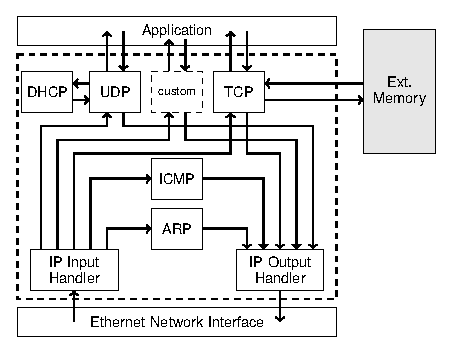
\includegraphics[scale=1]{introduction/fccm2015.eps}
\caption{The architecture of the Xilinx 10Gbps TCP/IP stack introduced in
\textit{Scalable 10Gbps TCP/IP Stack Architecture for Reconfigurable Hardware,
in FCCM’15}\cite{sidler2015tcp}.}
\label{fig:fccm2015}
\end{figure}



\chapter{Background}

In this chapter, we will introduce the basic concepts of the Internet Protocol
Suite, briefly describe its origin, semantics, and some of its protocols.
Furthermore, SME and the hardware it will run on will be introduced as a basis
for the implementation.


\section{Internet Protocol Suite (TCP/IP)}
Internet Protocol Suite, better known as simply TCP/IP, is a conceptual
model providing end-to-end communication between computers. It consists of
a collection of protocols specifying the communication between multiple
Internet systems\cite{RFC1122}.  The very early research and development
on what would later become the Internet Protocol Suite began in the late 1960s
by the Defense Advanced Research Project Agency (DARPA), and was being
adopted by DARPA, as well as the public, since 1983\cite{DARPA_internet}.
Although the Internet Protocol Suite predates the newer, arguably more
refined Open Systems Interconnection (OSI) model, TCP/IP still
remains the popular choice in modern systems.  As opposed to OSI 7-layer
model\cite{X.200}, the collection of protocols in TCP/IP are organized
into 4 abstraction layers, each related to their scope of networking
involved.

\subsection{Link Layer}
The link layer is the lowest, bottom-most layer in the Internet Protocol Suite.
Link layer addresses methods and protocols operating on the link that the host
is physically connected to\footnote{Wireless connections are also included
under this category.}. Contrary to the OSI model, this lowest layer in TCP/IP
does not regard the standards and protocols of the physical mediums used (the
pin layout, voltages, cable specifications etc.), making TCP/IP hardware-independent.
As a result, TCP/IP can in theory be implemented on virtually any hardware
configuration, emphasizing the flexibility of the model.

\subsection{Internet Layer}
The internet layer mainly concerns itself with sending data from the source
network to the destination network. This seemingly simple task requires multiple
functions from the layer:
\begin{itemize}
    \item Addressing and identification
    \item Packet routing
    \item \emph{Basic} transmit diagnostic information
    \item Carrying data for various upper layer protocols
\end{itemize}


\subsection{Transport Layer}
The transport layer establishes end-to-end data transfer between hosts.
Protocols in the transport layer can provide additional services to the user,
such as reliability, ordering, error- and flow-control, application addressing
(port numbers), error-checking, and so on.\\
While it is possible to bypass the protocols in this layer on most modern
network stacks, the protocols in the transport layer provide such essential
and useful services that it hardly ever makes sense to implement in the
application layer.\\
While there are numerous protocols defined in the Transport Layer, perhaps the
most well-known protocol in the stack is the Transmission Control Protocol (TCP).
Being one of the most used transport protocol for its reliability and congestion
control systems, it is rightly justified to refer to the whole Internet Protocol
Suite as simply "TCP/IP".


\subsection{Application Layer}
The application layer protocols are used by applications and services to
exchange information over the network. A few of the well-known application
layer protocols are the Hypertext Transfer Protocol (HTTP)\cite{RFC1945},
File Transfer Protocol (FTP)\cite{RFC0114}, and Simple Mail Transfer Protocol
(SMTP)\cite{RFC0788}.\\
This layer is usually implemented by the userspace applications themselves, and
therefore are not strictly required to actually run a TCP/IP network.



\section{Hardware}
The networking stack is intended to be flexible enough to run on just about any
configuration of hardware and software. However, this also means that it cannot
depend on any major external components, such as an existing memory, a processor,
or any form of operating system. Fundamentally, not only the software-part of the
networking stack has to be implemented, but the hardware needs to be defined
as well. This hardware should be self-contained enough to work well in combination
with any additional system, which the user incorporate for networking.\\
A wide variety of hardware types exist for such independent system, such as
Application-specific Integrated Circuit (ASIC), Complex Programmable Logic
Device (CPLD), Socket on a Chip (SoC), and Field-Programmable Gate Array (FPGA).
Each of these integrated circuits have their advantages and disadvantages; some
of them are re-programmable, some are cheap and disposable, and some are excellent
for general-purpose applications.\\
In this thesis, only FPGAs will be taken into consideration for its re-programmability,
its fairly low-cost, and the compatibility with SME code-generators.


\subsection{Field Programmable Gate Array (FPGA)}
Field Programmable Gate Arrays, or FPGA for short, are devices containing
integrated circuits (ICs) consisting of arrays of logic blocks.
These logic blocks can be programmed to form arbitrary logic circuit by simply
synthesizing a design and then loading it onto the board. This process alone
can save the manufacturer months by not having to fabricate a whole new IC. \\
FPGAs can be used for any computational tasks without the need of any additional
hardware. Usually, these devices are used for smaller, domain-specific tasks,
where the control over the hardware yields significant performance increases.
FPGAs are indeed very universal, and can be used in product-design, prototyping,
as well as in final products. Products like car driver assistance
systems\cite{xilinx_fpga_automotive}, audio decoders\cite{xilinx_fpga_audio},
or even internet search engines\cite{bing_search_fpga}  all utilize FPGAs to
increase the performance, lower the electrical bill, and  boost the development
potential.


\subsubsection{Technical specifications}
Field Programmable Gate Arrays consists of a vast number of ICs, which can
be reprogrammed at any time for a desired application or functionality\cite{ni_fpga},
making the devices very flexible and extensible, even after manufacturing.\\
These ICs are practically totally independent, and their logic within can be
programmed and combined in virtually any way with other ICs. This, however,
poses a problem, as signals do not propagate through circuitry, immediately, but
rather, they have a slight delay.
Sometimes, two events precede each other, while other times, events of distinct
timings must occur simultaneously.
Since the order of events is critical for correct and expected execution in
digital circuits, a digital clock is used to ensure everything runs in sync.
A clock in this context emits a series of pulses in a pre-determined and very
precise interval. These pulses are used to control the execution of various
elements in the circuitry.\\
When synthesizing to a FPGA, the compiler finds the longest code-path, it finds
the required circuitry to perform the calculation, and then it determines the
minimal required time for the signals to propagate through the path. In this
manner, the fastest possible clock can be found for that particular circuit.\footnote{
    Although many modern FPGAs consist of multiple regions which can have individual
    clock-rates. While it is a demanding task to propagate signals across these
    boundaries, a performance increases can be gained.
}
With innovations and steady improvements in modern FPGAs, the circuitries within
the devices can be clocked at higher than 500 MHz\cite{xilinx_fpga}.



\subsubsection{Programming an FPGA}
Unlike conventional processors with a very sequential nature, the logic blocks
in FPGAs are truly parallel in nature. Given the right programming, an FPGA can
allocate dedicated sections of the chip for each independent subtask, enabling
the circuitry to perform numerous independent calculations at once\cite{ni_fpga}.
Unfortunately, this universality of FPGAs comes at a cost to their performance.
Whereas conventional processors are heavily optimise based on the predetermined
circuitry, FPGAs programmers must ensure to utilize the parallel nature of the
device in order to secure best possible performance. Even worse, the FPGA must
be programmed in such a way that all paths in the electrical wiring can be
in any time-frame.\\
Due to this parallel nature of FPGAs, conventional programming languages are
next to impossible to use. To define the behavior of an FPGA, Hardware
Description Languages (HDL) are used. These programming languages are not easy
to learn without a good grasp of electrical engineering. Even with prior
programming knowledge, the unusual approach to concurrency in these languages
can be hard to understand for average developers.\\
To simplify the development process, most manufacturers offer predefined
circuits along their FPGAs. These predefined circuits are more commonly known
as Intellectual Property (IP) cores, and can provide the hardware designers
with pre-made circuitry for a wide variety of functionality. While most IPs
provide the functionality of processors for testing on an FPGA, mp3 audio
decoding or PCI bus interconnect can be obtained as well\cite{fpga_for_dummies}.



\section{Synchronous Message Exchange}
The Synchronous Message Exchange
model (SME) is a messaging framework created in order to help model
hardware descriptions\cite{sme_for_hardware_designs}.  It was conceived
once the flaws of using Communicating Sequential Processes (CSP) was
identified during the modelling of a vector processor with CSP using
PyCSP\cite{PyCSP}.  It turned out that there is a major discrepancy
between the way data is propagated in hardware opposed to that of the
CSP model. While CSP does not pose any requirements on the communication
between processes, in digital hardware, all communication has to be
synchronized, driven by a clock. To combat this in the CSP model, a
global clock process needed to be implemented, which was connected to
all other processes. Additionally, latches had to be introduced in order
to not overwrite values during a cycle. This caused an explosion of both
channels and latches in the final design, making CSP a much less viable
framework for hardware modelling\cite{sme_for_hardware_designs}.

\subsection{The model} The SME model consists of only a few fundamental
concepts. Each SME model is a \textit{network} consisting of one or more
\textit{processes}. These processes do not share any memory or storage,
but are interconnected with \textit{busses}.  These busses are perhaps
the most interesting units in SME model, as they not only propagate
information between processes using the underlying \textit{channels},
but also introduce an implicit clock between the processes.\\

\subsection{Process execution flow} The execution flow of a process is
fairly simple, and relates very closely to that of the actual hardware. At
the beginning of a clock-cycle, the input-ports are read into the busses
they are connected to. Then, the process executes its "compute" stage, and
the results, if any, are written to the output-port, which will be read
by the following bus. A visualization of the execution flow can be seen
on figure \ref{fig:sme_clock}.  \pic{0.5}{background/sme_clock}{An
illustration of a typical SME clock-cycle}{fig:sme_clock}
It is important to note that although certain channels might be written earlier
than others in a process clock, the subsequent processes connected to said bus
will first see the values change in the beginning of the next clock cycle.


\subsection{Using SME}
SME has undergone multiple iterations, reworks, and extensions. While
it is still under very active testing and development, its core
functionalities and features
 are well-established and stable\cite{bus_centric_sme}.\\
SME has concurrent implementations in the C\# and Python languages,
with promising efforts to unify these under a common intermediate
domain-specific language SMEIL\cite{smeil}. The C\# version has
exhibited various advantages over the Python counterpart, such as
the more error-prone strong typing system, which better reflects the
functionality of the hardware, as well as making the code more readable to
the programmer. At the time of writing, the C\# implementation currently
enjoys the most recent features of the SME model, as it is being the
most actively developed version.




% Chapters:
% - Network stack architecture
\chapter{Design}
\label{chap:design}
% introduction about the network stack?

\section{Overview}
The networking stack introduced in this thesis is implemented in the C\#
programming language with SME. The aim of its design is to capacitate performance,
flexibility, and ease of use. In this chapter, the design principles are
described, the architecture of the solution is outlined, and the components are
outlined.


\subsection{Design principles}
As briefly mentioned in the introduction, the proposed network stack is to
provide an alternative to the existing proprietary network offloading engines.
While the main goal of this thesis is to research and study the suitability of
SME for implementing a TCP/IP stack on an FPGA, there are many other aspects of the
system to be studied.\\
The extensibility of the network stack are to be tested by studying the effects
of introducing new protocols to the stack. While the network stack should be
able to be refined with new and custom protocols, it is to be studied which
implications it has for the system. Mainly, it is to be seen how the addition
of new protocols affect the performance, scalability, and viability of the
system.\\
In the same vein, the design should be as FPGA-agnostic as possible. While this is
mainly guaranteed by the SME framework used to develop the system, the underlying
systems, operations, and features should be easily portable across FPGA manufacturers.\\
Lastly, the design of the networking stack should be interoperable with other
systems on the FPGA, or even FPGAs. It is to be seen how easy it us to modify
and extend the versatility of the system without any major modifications or
even extensible knowledge of the system. As an example, the networking stack
can be expanded with a firewall, developed alongside this project.

\subsection{Initial requirements}
Following our design principles, initial requirements and goals for the
networking stack are set so that these can be tested and improved upon.
\begin{itemize}
\item \textbf{Essential protocols only}\\
Considering that the SME project is still fairly early in its development, and considering
the sheer number of protocols in the internet protocol suite, the networking
stack in this thesis is to support only the absolutely essential protocols
required to provide the users with a meaningful interface to the internet.
These protocols should be picked such that the system can provide the end-user
with a network data-stream, which can transport information to and from a remote
computer.\\
The initial protocols chosen may be implemented and supported partially, but
they must not deviate from the standard specifications.

\item \textbf{Support an interface for the end-user}\\
The system must be controlled by an end-user on the FPGA. Such an interface is
very unique in its own way, compared to standard software interfaces, like the
ones defined in the POSIX collection of specifications. By supporting such an
external interface gains insight in the way such a networking stack will be used,
and which measures must be taken in order to provide the best possible integration
and performance considerations.

\item \textbf{Independent of underlying physical hardware}\\
By using SME, the underlying hardware description language code can be abstracted
away from the actual implementation. This will later provide developers to easily
modify and tweak the networking stack without having to consider the target
hardware.\\
Likewise, the networking stack may not rely on using a certain physical layer hardware,
and must be designed to be independent of the underlying hardware used for the
physical connections. This will ensure that the target hardware can easily
swap between physical connectors, such as going from ethernet cables to wireless,
or even another FPGA.
\end{itemize}

\section{Initial design}

% Spans 2 columns
\begin{figure*}
    \centering
    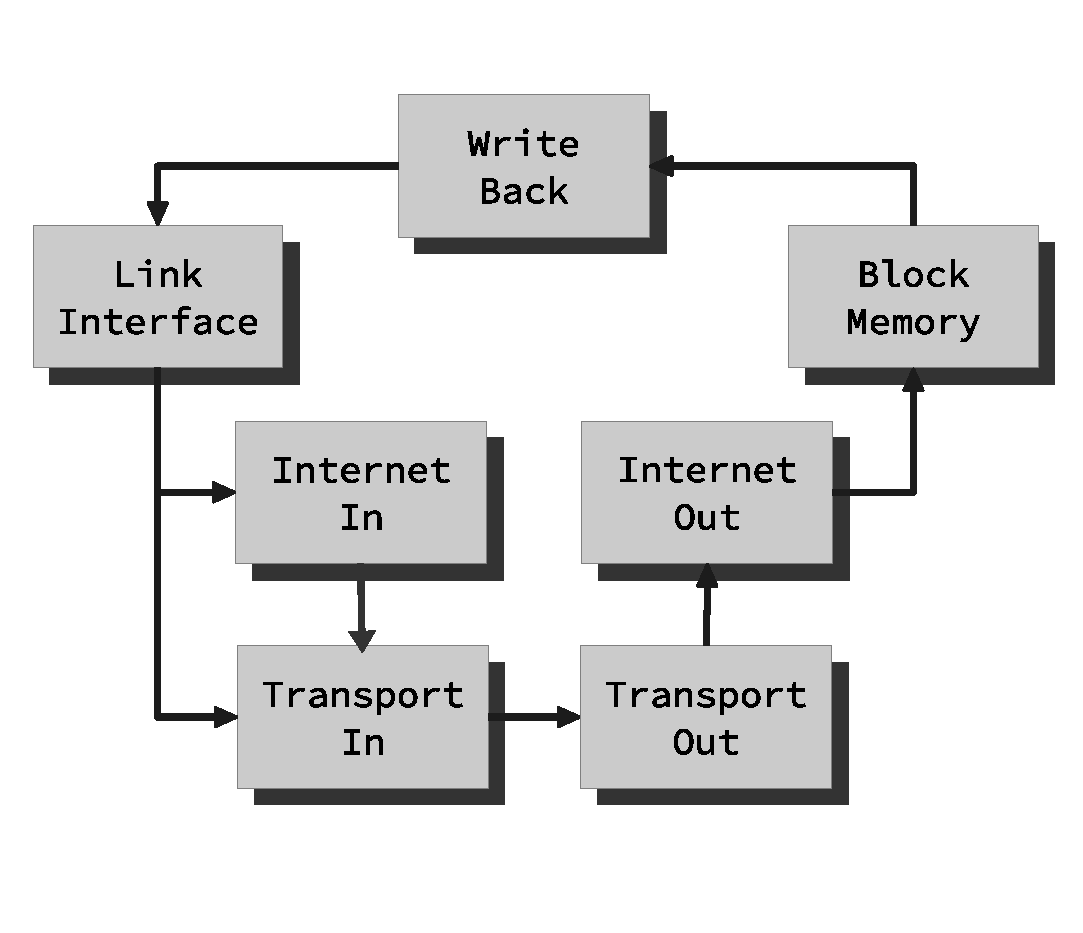
\includegraphics[scale=0.45]{design/design_0.eps}
    \caption{The initial design}
    \label{fig:initial_design}
\end{figure*}

The initial architecture had a very simplistic approach to its design in order
to aid with early identification of potential issues and problems.
The basic idea of the initial design is to minimize the number of memory
operations carried out. Under the assumption that the Ethernet interface used in the network
stack will likely have limited memory, everything needs to be copied directly to
the stack. Figure \ref{fig:initial_design} shows the initial design, where the
leftmost module Ethernet connects to the memory for direct access, and each
parsing layers listens to this connection and performs accordingly. Each parsing
layer also connects to the subsequent layer in order to flag when the subsequent
layer should start listening on the data-bus (that is, where the current packet
header stops and the next header begins).\\
An advantage that this design provided was the cetralized memory, which is much
easier to up-scale in terms of capacity and bandwidth. This global memory would
also be able to modify packets in-place, removing duplicate data, minimizing the
need to copy data around, and making it easier to keep track of the memory
fragmentation.

\subsection{The issues}
As anticipated, this initial design brought fourth the main issue fairly quickly
in the implementation phase, where most of these stem from the differences in
programming hardware as opposed to the software network stack, from which the
inspiration was drawn.

\subsubsection{Internal parsing buffer or memory is largely unavoidable}
Although listening to the global data-bus and processing on the bytes currently
therein  seems like an efficient way of minimizing the data-transfer required
across processes, it has shown to yield some unavoidable challenges.\\
Parsing fields in a packet-header is much more cross-dependent than initially
anticipated; each field might have numerious implications on the way preceeding
and subsequent fields are read and interpreted. As an example, in the Internet
Control Message Protocol (ICMP), a redirect message type has an IPv4 address field in
the header, whereas in the timestamp message type, this field is interpreted as
both an identifier and a sequence number.
This sort of inter-dependency is hard to parse without the ability of caching
or buffering the header locally in the parsing process.

\subsubsection{Overutilized memory module}
While the ethernet is the main writer to the memory module, the parsing layers
need to access and write to the module as well. At the very least, the memory
module would have 6 connections in the network, not counting any additional
components, such as user interface, firewall, etc.
Although numerous memory implementations exist on the FPGA landscape, Block RAM
(BRAM) seems to be the most suitable in this situation for its speed and latency.
Unfortunately, many widely used block RAMs only have 2 simultaneous connections
(or "ports") at the same time. Additionally, the block rams are frequently
limited to only operate a few bytes of data at a time.\\
Although some block RAMs, such as the ones found in Xilinx FPGAs can be cascaded\cite{xilinx_fpga_memory_resources}
to lessen the impact of these limitations, this hardly provides a good basis for
a scalable design.

\subsubsection{Data fragmentation and memory management}
Another problem a unified address space in the global memory is how costly
basic memory operations, such as moving or copying, become. The initial
assumption that packets stored in memory could be reused by modifying them
in-place and send them turned out to be misguided, since the layout, size, and
the number of the outgoing packets very rarely resemble the in-going packets.\\
Furthermore, the general purposeness of the memory makes it very hard to
structure. Without very complex memory management, the memory can get very
fragmented and slow.


\section{Revised design}
The initial architecture focused heavily on the input from the link interface,
minimizing hardware memory requirements, and to minimize the latency from the
source data-stream to its respective layer handler. Unfortunately, the opposite
revealed to be true, as the overly-utilized memory unveiled plentiful issues to
the performance.\\

\begin{figure}[h]
    \centering
    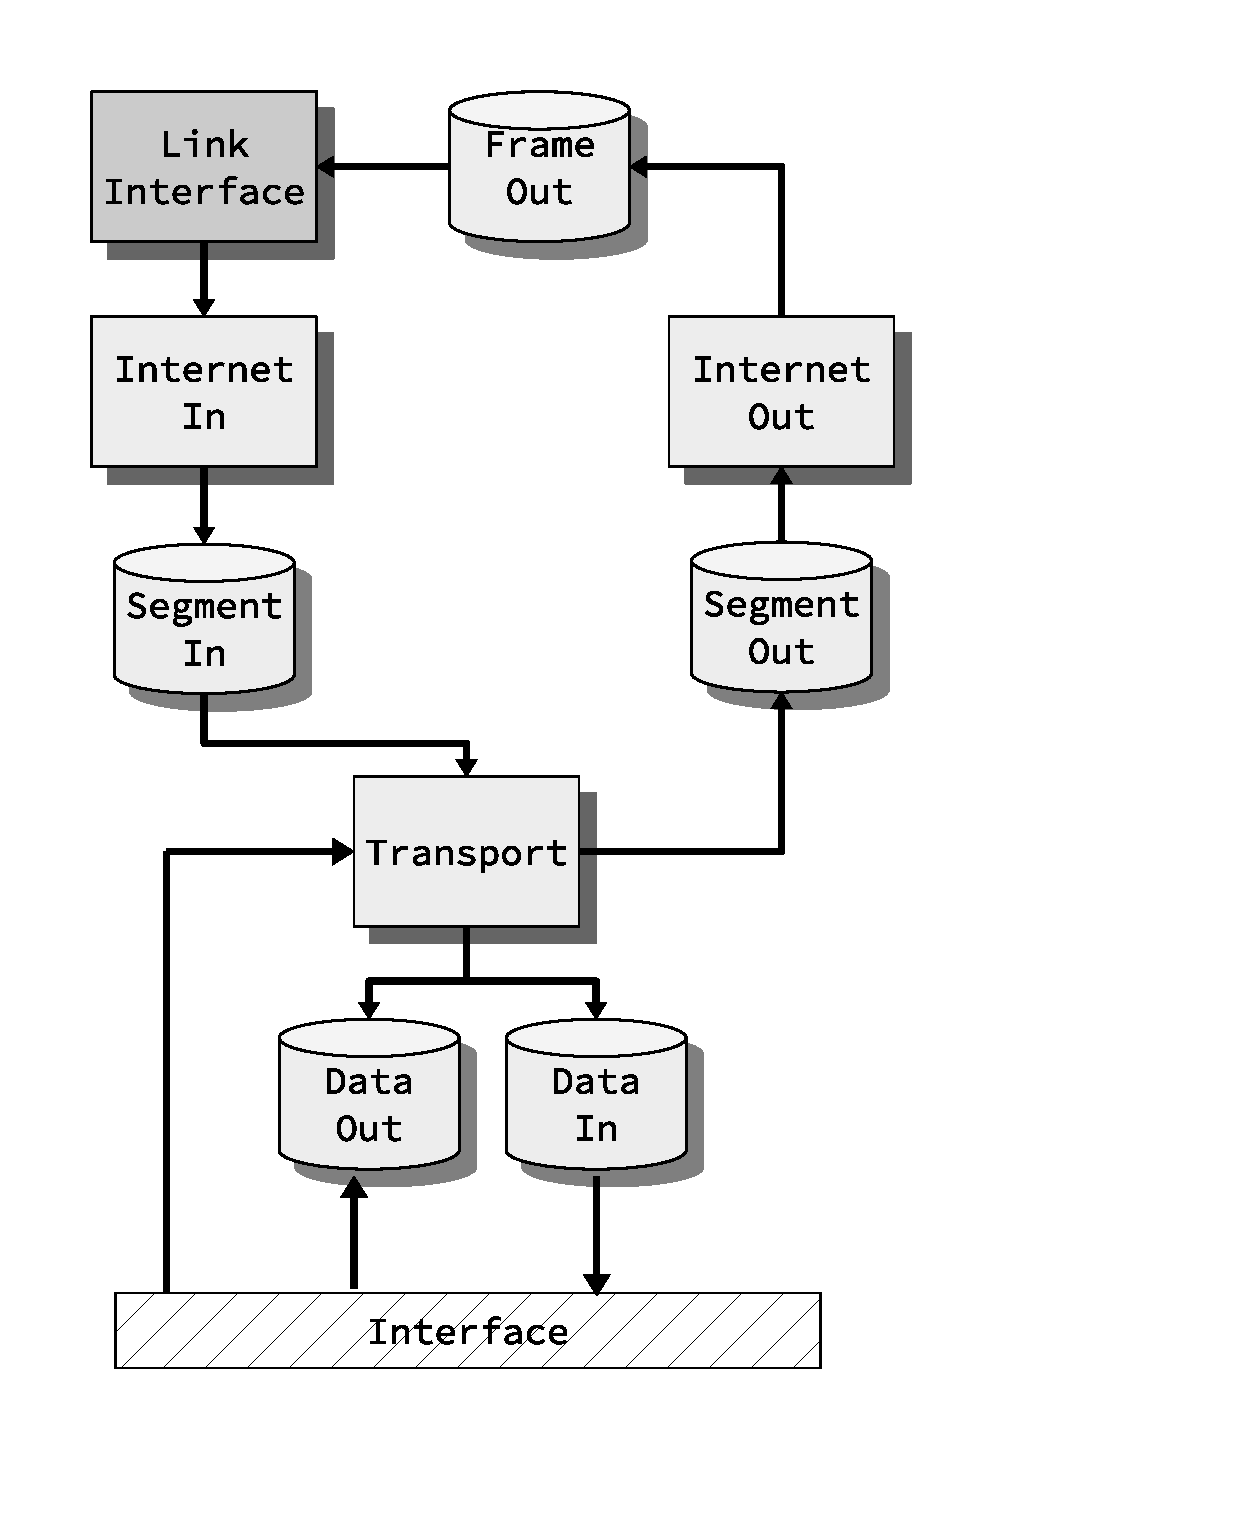
\includegraphics[scale=0.45]{design/design_1.eps}
    \caption{Second iteration of the design}
    \label{fig:second_design}
\end{figure}

To avoid the problem with global memory, the data needs to "flow" through the
components that need the data at that time. Therefore, as opposed to the initial
design, where the link interface writes to memory directly, in the revised design,
this connection is completely removed. The idea is to let all the data pass
pass through each state, letting each stage parse the required information, and
passing the rest to the next components.\\
As seen on figure \ref{fig:second_design}, the link interface, which
provides the raw byte-stream from the network, is connected to all of the input
parsing layers. The layers are connected in the order in which a network frame
is parsed; link- to internet- to transport-layer. This approach aims to utilize
the fact that the layers can act immediatelly upon the packets received directly
from the source, avoid having to buffer the whole packet in each stage, as well
as easing the logic required to buffer the data across the layers.\\
This design starts by the Link Interface sending one byte at a time through its bus.
The \texttt{Link In} will parse the first header, and signal the next layer upon completion.
\texttt{Internet In} will then start to listen on the \texttt{Link Interface} bus
and, using the information from \texttt{Link In}, parse the internet header
accordingly. The same procedure would be applied to the connection between
\texttt{Internet In} and \texttt{Transport In}.\\
When data is to be sent to the internet, the network frame would be built bottom
up from the transport layer through internet to the link layer.

\subsection{The issues}
The issues quickly surfaced during the implementation of this revised design. Although
the interconnect from the \texttt{Link Interface} to all the subsequent layers
in parallel promised negligible latency, it came with a great cost to the solution.

\subsubsection{Process under-utilization} \label{item:process_utilization}
Since each "in" process has to wait for the previous layer to signal when to
start listening on the data-bus, the layers would in average only be active a third
of the time. Since each layer has very little information about the states of
the other layers, it would become a challenge to get any other work done during
these phases.\\
For example, it would be an immense challenge to coordinate an ICMP reply on a
faulty packet in the \texttt{Internet In}.

\subsubsection{Redundant Link layer}
While the Link layer is an essential part of the Internet Protocol Suite, it did
not fit well with the functionality of the rest of the stack.
Most network interfaces are equipped with buffers, on which integrated circuits
perform operations such as error check using cyclic redundancy check, de-noising,
timeslot management, etc.
Likewise, the Pmod NIC100 Ethernet interface has built-in controller with
internal memory suited for buffering the incoming packets\cite{microchip_enc424j600}.
This memory, apart from the cyclic redundancy check, can be used as the initial
step for parsing the packet, and only send the datagram to the stack.


\subsubsection{IPv4 fragmentation and out of order TCP packets}
The chaotic nature of internet routing might cause packets to come out of order,
or even get fragmented along the way. Since each layer parses the packet immediatelly
as it is written to the bus, it became a challenge for the layers to figure out
what to do. On IPv4 fragmentation, if the second half of a dataframe arrived
first, the Transport header would not be available to the Transport layer.
Although IPv4 fragmentation is an increasingly rare phenomenon, the network
design is not able to handle the situation well.


\subsubsection{TCP connection state sharing}
With a clear separation between the "in" layers and the "out" layers, the
Transport block had to be split as well. Unfortunately, unlike the other stateless
layers, the transportl layer actually needs to keep track of the connections and
their states. On every segment received, the appropriate connection needs to be
updated accordingly.\\
In the TCP protocol, the connection state changes on both receiving and sending.
In this case, the \texttt{Transport In} and \texttt{Transport Out} have to
agree on a shared state. As these states can be quite large, and the should
support multiple connections at once, one large bus containing all the information
is not feasible. To solve this, a negotiation protocol may be introduced, however,
as pointed out in item \ref{item:process_utilization}, the processes are very
limited in their execution time. A negotiation would be very hard to achieve in
such circumstances.


\subsubsection{Problematic order of building and sending outgoing packets}
Outgoing packets are built in the reverse order of which they are parsed -- the
inner layers are built first, and then the packet grows outwards by adding new
layers on top of the existing one.\\
That in itself is not a problem, as the packet can be easily passed through the
network backwards from the last byte first. That is, the inner-layer of a packet
is passed on to the next layer first, then the header packet header is built,
and lastly, the header is passed on backwards.\\
However, this assumes that the next layer to process the packet is available at
all times in order to process the packet. This is certainly not the case, as
layers such as \texttt{Link Out} and \texttt{Internet Out} might be in the
process of sending out their own protocol-specific control messages (such as
an ARP annoucement in the Link Layer or ICMP reply in the Internet Layer).\\
A negotiation protocol can be implemented between the outgoing processes in to
postpone the outgoing packet, but these structural hazards, as known from
conventional processor pipelines, add a lot of complexity to the system.





% \subsubsection{Control and logic flow}
% Although the layers take turns to parse the incoming byte-stream, the design
% handles the whole packets at once. This leaves

\section{Pipelined design}
While it would be possible to work around these identified issues with the
revised design in the code, the
added complexity would have additional ramifications on the project as a whole.
Upon further analysis of analysis, it is clear that the source of the issues is
the parallel arrangement of the process blocks.

\begin{figure}
    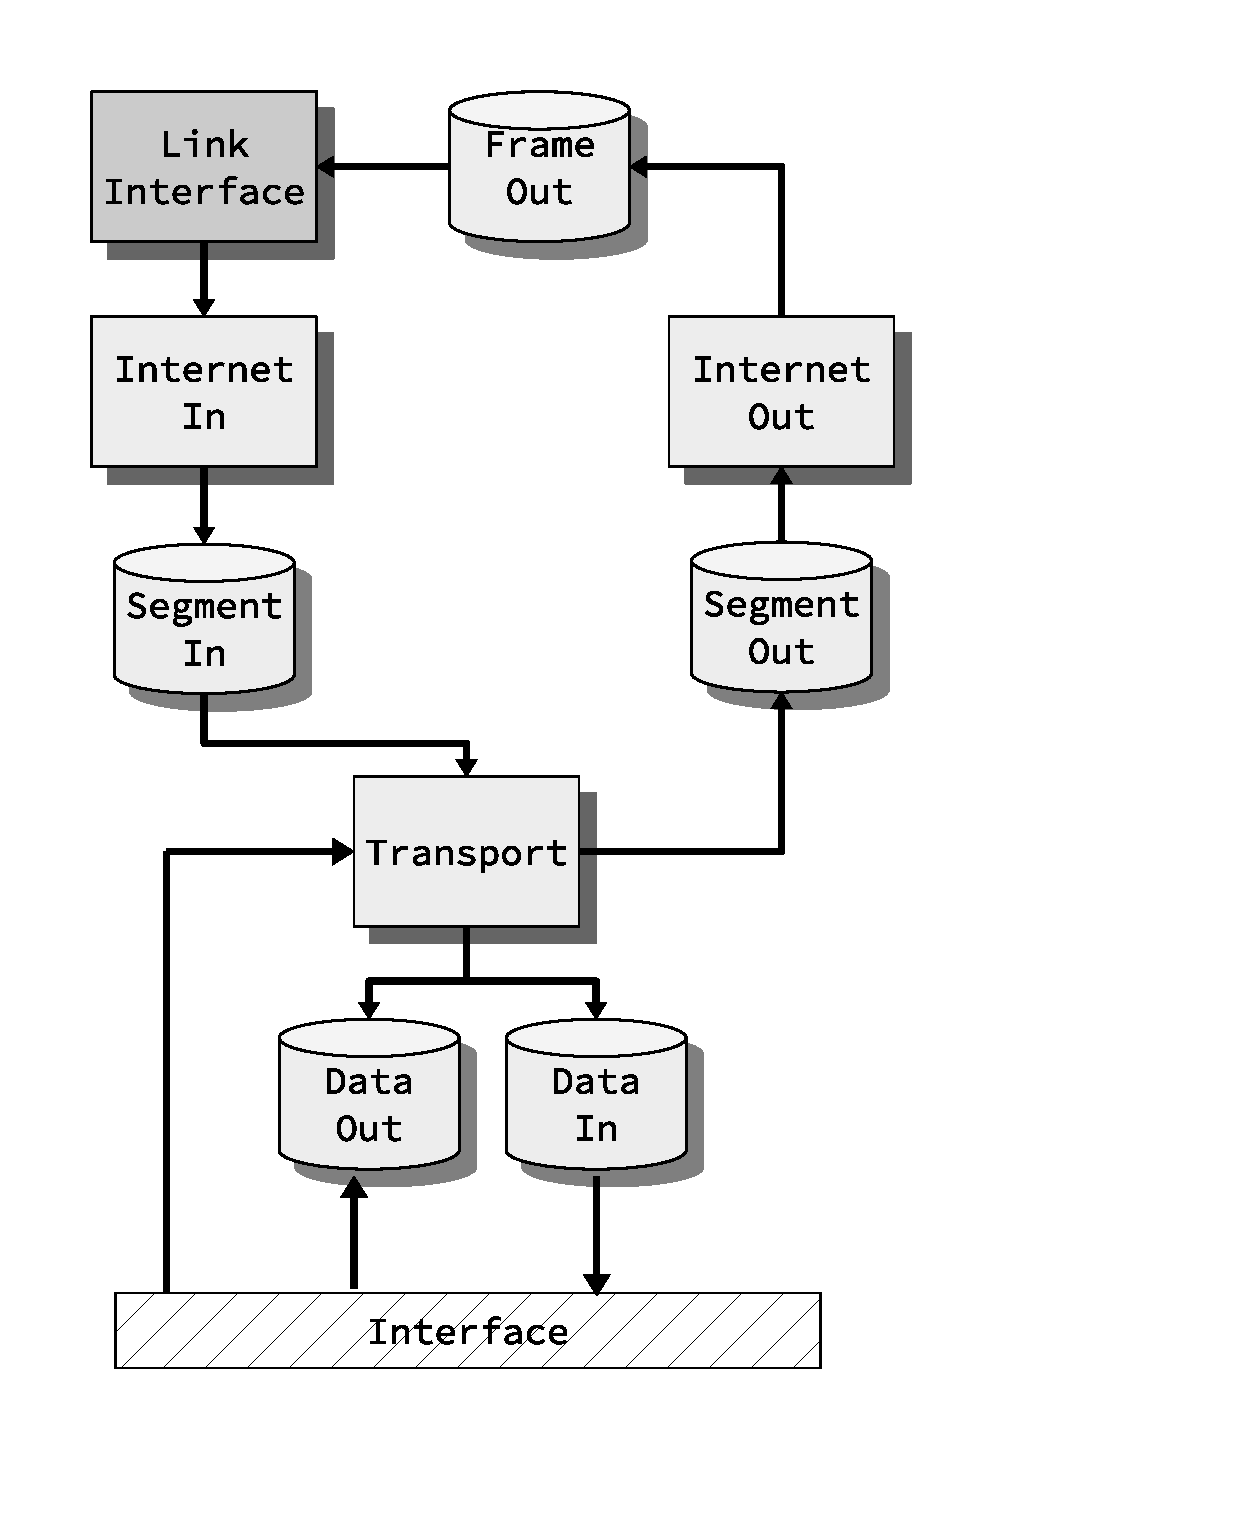
\includegraphics[scale=0.45]{design/design_2.eps}
    \caption{The final design. The rectangles represent "compute" processes,
while the cylinders represent the buffers.}
    \label{fig:final_design}
\end{figure}

The next iteration of the design utilizes a fairly standard approach to
pipelining, albeit with an unusual transfer of data between the stages.\\
The idea with the pipeline is to enable the processes to receive, compute, and
forward data at their own pace, without any major limitation from the other
parts of the system.

\subsection{Internet layer processes} \label{sec:layer_processes}
The processes performing computation and processing on the actual internet
packets, called "layer processes" for brevity, are by large kept intact from the
previous design. The fairly simple, but highly sequential nature of packet
header parsing turned out to be very complicated to optimise with the additional
computing power of the hardware, without introducing too much complication.\\
Missing from the updated figure \ref{fig:final_design} are the \texttt{Link In}
and \texttt{Link Out} processes, which, for now, are handled by the ethernet
interface, which can easily parse and strip the first frame headers.


\subsection{Busses}
The busses in the revised pipelined design are devised such that communication
is only limited to the immediate neighbours in the logical network. This design
is put in place so that the synchronization and the order of execution is much
easier to keep track of, so that fewer race-conditions occur, and so that blocks
in the network are easier to replace, remove, or modify, without having a large
cascade effect on the whole network, as opposed to only the neighbours.\\
Whereas in the previous design where the busses would simply write new data on
every new clock-cycles regardless of the reading processes, now there must be
some logic to actually ensure that the reading process is ready to receive new
data. While the Data Buffers, as introduced in the next section \ref{sec:data_buffers},
solve the issue of blocks reading and writing data at their own pace, the busses
must support an interface for sharing the state of both processes. Thus, while
the busses are depicted as directional with arrows in figure \ref{fig:final_design},
there is naturally a need for a control signal in the opposite direction to
control the data-flow. This communication protocol will be discussed further in
the implementation section \ref{sec:interface_signal_protocol}.


\subsection{Data buffers} \label{sec:data_buffers}
Illustrated as cylinders on figure \ref{fig:final_design}, First-In, First-Out (FIFO)
buffers are introduced between each parsing process in order to control the data-flow
between the layers. Apart from maintaining a fairly large memory bank through
the block-RAM, these buffers also contain logic to store the incoming data
intelligently in order to offload the following processes. For example, the
\texttt{Segment In} buffer ensures that fragmented IPv4 packets are defragmented
before leaving the buffer.
However, introducing a new "type" of a process --- the buffers --- poses a new
challenge. While the buffers can be read from at any time, the layer-parsing
processes do not have this luxury, as they do not have any significant internal
buffer. Here again it becomes obvious that a handshake protocol needs to be used
in the bus-communication between the buffers and the processes.

\subsubsection{Order of outgoing packets}
In the previous design, it was obvious how sending packets might become a challenge
given that all processes involved must be ready to promptly operate on the
outgoing packet. With the introduction of data buffers, the processing of an
outgoing packet can be delayed.
However, there lies another small problem with the way data is passed around.
The \texttt{data}-section has to be read by Transport in first-in, first-out
order, solely for the reason that Transport does not know beforehand how much
data to send, nor whether more urgent tasks appear during the transmission.
Figure \ref{fig:sending_packet_order} shows the possible ways of creating and
passing a packet along the network stack.
\begin{figure}
    \centering
    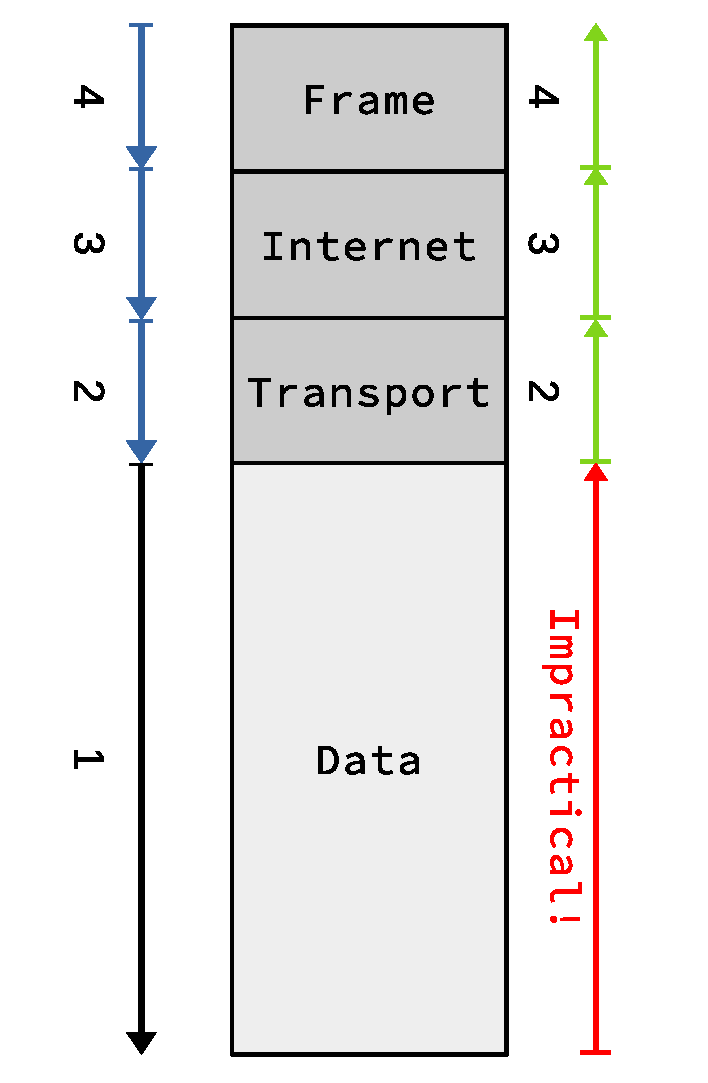
\includegraphics[scale=0.45]{design/sending_packet_order.eps}
    \caption{Possible orders of ways of building an outgoing packet}
    \label{fig:sending_packet_order}
\end{figure}
On the right side of figure \ref{fig:sending_packet_order}, the data is sent
from the last byte first, indicated by the red arrow from bottom up. Then, the
transport-, internet-, and lastly, the frame-header is built and sent with it
in the same order, from the last byte of the header till the first.
While this method is fairly simple, it has two problems that are hard to work
around -- firstly, the user might be in the process of writing outgoing bytes
to the \texttt{Data Out} buffer, in which case, Transport cannot beforehand
start sending the last byte. The second problem is that, although Transport
wants to send as much data at once as possible to lessen the overhead from the
rest of the package, more urgent tasks might come up during the transmission,
yet the operation has to finish reading the last (first) byte.\\
The left side of figure \ref{fig:sending_packet_order} shows another approach
to sending a packet. Here, the data portion of the packet is read as is in the
first-in, first-out byte order. The headers are written afterwards, also in the
FIFO order. It is important to notice that even though the package looks
structurally right when reading backwards (the frame header is in the beginning,
then Internet header and so on), the ordering of the bytes is not correct! For
example, if reading the right-hand on figure \ref{fig:sending_packet_order}
packet in reverse order, the data section would begin with the very last byte!\\
Here, the intermediate buffers once again offload this problem, as one of the
brilliant features is that they enable the system to pass bytes out of order.
In that case, the sending process can begin in the middle of a package, and then
append to the beginning of it at the very last.\\
Figure \ref{fig:sending_packet_graph} shows the building of an outgoing packet.
Between each process, the colored block represents the state of the packet
being passed along the processes. The red arrow indicated the first stage of
the connection between processes, where data is passed from a previous layer.
The blue line indicates the data that the process itself appends to the stream.\\
The implementation of this out-of-order forwarding will be described in-depth
in the implementation chapter \ref{chap:implementation}.

\begin{figure*}
    \centering
    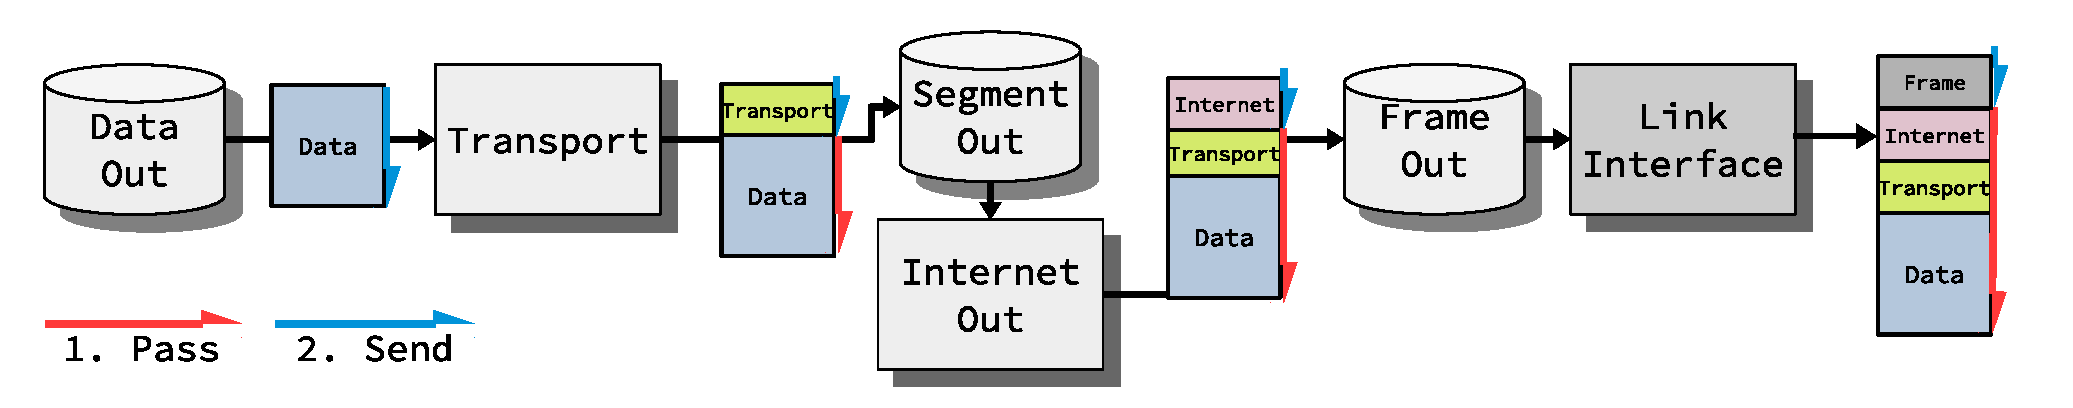
\includegraphics[scale=0.45]{design/sending_packet_graph.eps}
    \caption{The order in which an outgoing packet is built and passed through the network pipeline.
    The colored boxes represent the state of the outgoing packet, the red arrow
    indicates the first stage of forwarding, and the blue line indicates the last stage.}
    \label{fig:sending_packet_graph}
\end{figure*}



\subsection{Interface}
Lastly, the Interface is designed so that the end users and system can utilize
and use the network stack.\\
The networking stack is controlled with 3 connections (consisting of bus-pairs):
the control-, the read-, and the write-connection. While the last two connections
are incredible simple and only transfer data from the \texttt{Data} buffers,
the last connection controls the whole network-stack.

\subsubsection{Read/Write interface}
In conventional programming languages, the user would usually supply the a
function call with an array or a list on which the function can operate.
However, in hardware, this is generally not the case, as arrays are costly to
transmit at once.\\
Therefore, the two read and write interfaces would simply stream one byte at a
time, and it is up to the user to be prepared to read or write the data.


\subsubsection{Interface Control Bus}
The Interface Control Bus controls all the "business" logic of the network --
maintaining the active connections, starting and closing connections, and various
other protocol-specific control on each connection.\\
Currently, all this can be handled by the \texttt{Transport} block which has all
the necessary information to handle the interface requests.\\
The design of the Interface is based on the widely adopted Berkeley Sockets library,
which saw the first implementation in 4.2BSD, and has been defacto a standard
component in the POSIX specification\cite{tcpip_illustrated_vol2}. There are
multiple reasons for this decision:
\begin{itemize}
\item The Interface will feel more familiar to users accustomed to the Berkely
Sockets API commonly found in mainstream systems such as Linux, OSX, and BSD
variants.

\item The inner workings of the stack will be more transparent, and the API
exposes fairly fine-tuned control over the whole network stack.

\item Even with the relatively few functions exposed, the API
has thrived in the most used systems as of now. It would be an understatement to
say that the Berkeley Sockets API have stood the test of time, and therefore, it
is a good basis for the interface used in the network stack.

\end{itemize}

The first version of the stack should support the following functions:
\begin{description}
\item[\texttt{listen(protocol, port)}]\hfill\\
    Finds and initializes a free socket with the given protocol and port. This
    socket is immediatelly put into listen mode.
    Returns error if protocol is not supported, if port taken, or if no free sockets
    are available.
\item[\texttt{connect(protocol, ip, r\_port , l\_port])}]\hfill\\
    Connects to a remote endpoint on \texttt{ip:remote\_port} using \texttt{protocol}.
    This call is used mainly by connection-based protocols that need to
    establish a connection before exchangning data, although it can also be used
    by datagram-based protocols as a way of setting the default destination to
    send subsequent data to.
    Returns error if protocol is not supported, if no free sockets are available,
    or if the optional local port is taken.

\item[\texttt{accept(socket)}]\hfill\\
    Accepts the pending connection and sets up the underlying socket state
    accordingly. Note that unlike the POSIX implementation of \texttt{accept},
    which returns a new socket with the connection, this implementation changes
    the state of the current, listening, socket.
    Returns error if no pending connection to accept, or if invalid socket
    supplied.

\item[\texttt{send(socket, byte, [ip], [port])}]\hfill\\
    Queues a byte for sending through the socket. An optional IP address and
    port can be specified in certain connectionless protocols.
    Guaranteed to succeed, given that the transport-bus can be written to. More
    on this discussed later.
\item[\texttt{recv(socket)}]\hfill\\
    Reads (or "receives") a single byte from the socket. The appropriate error
    code is set if no byte available on that particular socket.

\item[\texttt{close(socket)}]\hfill\\
    Closes the connection on \texttt{socket} and frees the socket for further
    usage. Calling on an already closed on non-existent socket has no effect.
    Guaranteed to succeed.

\end{description}

While the arguably most essential functions have been defined, there are some
functions from the Berkeley Sockets API that have been omitted for purely
technical and practical reasons.\\
The function \texttt{socket()} is mainly used to allocate and create new sockets
in an environment, but given that the hardware network stack has static allocation
of the sockets, it is not needed.\\
Additionaly, the \texttt{bind()} function is also missing for the sole reason
that in the current implementation of the network stack does not have any valid
reason not to bind a socket immediatelly.


% \cofeAm{0.7}{0.75}{2}{80}{0}





% - Data buffering and IO
% - Network API and interfacing
% - Test setup
%   - Code tests (simulations)
%   - FPGA
%   - Real applications
% - Results and discussion
% - Conclusions
% - Future Work




\newpage
\clearpage % force new page(?)
\newpage

\onecolumn

\appendix
\begin{appendices}

\end{appendices}

\newpage
\bibliography{bib}{}
\bibliographystyle{plain}


\end{document}
